\documentclass[9pt]{extarticle}

\usepackage[a4paper,landscape,margin=8mm]{geometry}
\usepackage[T1]{fontenc}
\usepackage[default]{sourcesanspro}
\usepackage[scale=0.92]{sourcecodepro}
\usepackage{multicol}
\usepackage{xcolor}
\usepackage{tikz}
\usetikzlibrary{positioning,arrows.meta,calc}
\usepackage[most]{tcolorbox}
\usepackage{enumitem}
\usepackage{tabularx}
\usepackage{booktabs}
\usepackage{listings}
\usepackage{array}

\pagestyle{empty}
\setlength{\parindent}{0pt}
\setlength{\parskip}{2pt}
\setlength{\columnsep}{9pt}
\setlength{\columnseprule}{0pt}
\renewcommand{\arraystretch}{1.12}
\setlength{\tabcolsep}{3pt}

% Chapter colours, matching the GitHub badges
\definecolor{orm}{HTML}{0969DA}
\definecolor{rmap}{HTML}{1A7F37}
\definecolor{norm}{HTML}{9A6700}
\definecolor{sql}{HTML}{CF222E}
\definecolor{care}{HTML}{6E7781}
\definecolor{ink}{HTML}{1F2328}
\definecolor{muted}{HTML}{57606A}
\definecolor{warn}{HTML}{BC4C00}
\color{ink}

\setlist{nosep,leftmargin=*,labelsep=3pt,itemsep=0.5pt}
\setlist[itemize]{label={\color{muted}\textbullet}}

% Topic box
\newtcolorbox{topic}[2]{%
  enhanced, colback=white, colframe=#1, coltitle=white, colbacktitle=#1,
  title={\bfseries #2}, fonttitle=\small,
  boxrule=0.7pt, arc=2pt, left=4pt, right=4pt, top=3pt, bottom=3pt,
  toptitle=1pt, bottomtitle=1pt, before skip=0pt, after skip=5pt}

% Subheading inside a box
\newcommand{\sub}[2][ink]{\par\smallskip{\color{#1}\bfseries #2}\par\nobreak\vspace{1pt}}

% Exam trap callout
\newtcolorbox{trap}{%
  enhanced, colback=warn!6, colframe=warn!6, borderline west={2pt}{0pt}{warn},
  boxrule=0pt, arc=0pt, left=4pt, right=3pt, top=2pt, bottom=2pt,
  before skip=3pt, after skip=3pt, fontupper=\footnotesize}

\lstdefinestyle{sql}{
  language=SQL, basicstyle=\ttfamily\footnotesize, keywordstyle=\color{sql}\bfseries,
  commentstyle=\color{muted}\itshape, stringstyle=\color{rmap},
  morekeywords={REFERENCES,ENUM,AUTO_INCREMENT,EXCEPT,ROLE,REVOKE,GRANT,COMMIT,ROLLBACK,START,TRANSACTION,IF,EXISTS,DEFAULT,LIMIT},
  columns=fullflexible, keepspaces=true, showstringspaces=false,
  aboveskip=2pt, belowskip=2pt, xleftmargin=2pt, frame=none,
  backgroundcolor=\color{sql!4}}
\lstset{style=sql}
\newcommand{\code}[1]{\texttt{\small #1}}

% ORM drawing helpers
\tikzset{
  ent/.style={draw=orm, fill=orm!8, rounded corners=2pt, minimum height=5.5mm, inner sep=2pt, font=\scriptsize\bfseries, align=center},
  val/.style={draw=rmap, dashed, fill=rmap!6, rounded corners=2pt, minimum height=5.5mm, inner sep=2pt, font=\scriptsize, align=center},
  role/.style={draw=muted, fill=white, minimum width=4mm, minimum height=3mm, inner sep=0pt},
  bar/.style={line width=1pt},
  dot/.style={circle, fill=ink, inner sep=0pt, minimum size=3pt},
}
% A binary predicate: two role boxes starting at (#1)
\newcommand{\pred}[2]{%
  \node[role, anchor=west] (#2a) at (#1) {};
  \node[role, anchor=west] (#2b) at (#2a.east) {};}

\begin{document}
\small

% ---------------------------------------------------------------- title strip
\begin{tcolorbox}[enhanced, colback=ink, colframe=ink, coltext=white, arc=2pt, boxrule=0pt,
  left=6pt, right=6pt, top=3pt, bottom=3pt, after skip=6pt]
{\large\bfseries IFB105 Database Management: Exam Cheat Sheet}\hfill
{\small ORM \;\textbar\; RMapping \;\textbar\; Normalisation \;\textbar\; SQL \;\textbar\; CARE}\hfill
{\small Minh Kha (Marvin) Truong, SSP}
\end{tcolorbox}

\begin{multicols*}{3}

% ================================================================ ORM
\begin{topic}{orm}{1 \quad ORM and the CSDP}
ORM = \textbf{Object Role Modelling} (not Object Relational Mapping).

\sub[orm]{CSDP steps 1 to 5}
\begin{enumerate}
  \item Turn examples into \textbf{elementary facts}.
  \item Draw \textbf{fact types} and do a \textbf{population check}.
  \item \textbf{Combine} entity types; mark \textbf{arithmetic} derivations \textbf{*}.
  \item Add \textbf{uniqueness} bars; check \textbf{arity}.
  \item Add \textbf{mandatory} dots; mark \textbf{logical} derivations \textbf{*}.
\end{enumerate}

\sub[orm]{Notation}
\begin{center}
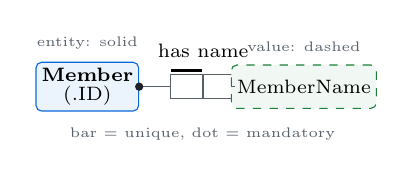
\begin{tikzpicture}
  \node[ent] (m) at (0,0) {Member\\[-1pt]{\mdseries (.ID)}};
  \pred{1.05,0}{p}
  \node[val] (n) at (2.75,0) {MemberName};
  \draw[muted] (m.east) -- (pa.west);
  \draw[muted] (pb.east) -- (n.west);
  \node[dot] at (m.east) {};
  \draw[bar] ($(pa.north west)+(0.4pt,1.5pt)$) -- ($(pa.north east)+(-0.4pt,1.5pt)$);
  \node[font=\scriptsize, above=2.5pt of pb.north, xshift=-2mm] {has name};
  \node[font=\tiny, color=muted, above=1pt of m] {entity: solid};
  \node[font=\tiny, color=muted, above=1pt of n] {value: dashed};
  \node[font=\tiny, color=muted, below=7pt of pa.south east, align=center] {bar = unique, dot = mandatory};
\end{tikzpicture}
\end{center}
\begin{itemize}
  \item \textbf{Entity type}: needs a reference mode, e.g.\ \code{(.ID)}, \code{(.Code)}.
  \item \textbf{Value type}: identifies itself (a string or number). Never has a reference mode.
  \item \textbf{Unit-based} modes \code{(AUD:)}, \code{(L:)}, \code{(cm:)} make an \textbf{entity} type.
  \item \textbf{Arity} = number of roles: unary 1, binary 2, ternary 3.
\end{itemize}

\sub[orm]{Step 1: elementary facts}
Pattern: \emph{entity type + reference mode + has/is + value type + value}.\\
\emph{The Member with ID `M01' has the MemberName `Ava Tran'.}
\begin{itemize}
  \item Can't be split without losing information.
  \item States something \textbf{true} (no ``is not'').
  \item Has \textbf{no conditions} (no ``if'', ``so'').
  \item A \textbf{tick-box} on a form is a \textbf{unary} fact, not a Yes/No value.
  \item Count \textbf{object types} only; not values or reference modes.
\end{itemize}

\sub[orm]{Step 2: population check}
Write 3+ sample rows under the role boxes.
\begin{itemize}
  \item Repeats in a column $\Rightarrow$ role is \textbf{not} unique.
  \item Object missing from a column $\Rightarrow$ role is \textbf{optional}.
  \item Can't fill a row $\Rightarrow$ fact type is wrong; go back to Step 1.
\end{itemize}
\textbf{Nest} a fact type (m:n bar) when facts are recorded about the pair itself, e.g.\ Booking \emph{was made on} Date.

\sub[orm]{Step 3: combine and derive}
Combine types if the same entity can be both, they are comparable, or you'd list them together. Use \textbf{role names} \code{[retailPrice]} to keep predicates apart. Derivable facts get \textbf{*} and a rule, and are \textbf{not stored}.
\end{topic}

\begin{topic}{orm}{1 \quad ORM: constraints (steps 4 and 5)}
\begin{center}
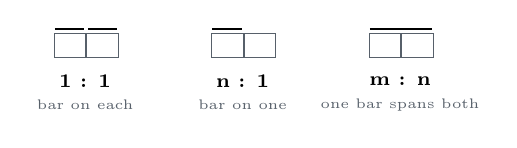
\begin{tikzpicture}[x=1mm,y=1mm]
  % 1:1
  \pred{0,0}{a}
  \draw[bar] ($(aa.north west)+(0.5pt,1.5pt)$) -- ($(aa.north east)+(-0.8pt,1.5pt)$);
  \draw[bar] ($(ab.north west)+(0.8pt,1.5pt)$) -- ($(ab.north east)+(-0.5pt,1.5pt)$);
  \node[font=\scriptsize\bfseries] at (4,-4.5) {1 : 1};
  \node[font=\tiny, color=muted] at (4,-7.5) {bar on each};
  % n:1
  \pred{20,0}{b}
  \draw[bar] ($(ba.north west)+(0.5pt,1.5pt)$) -- ($(ba.north east)+(-0.5pt,1.5pt)$);
  \node[font=\scriptsize\bfseries] at (24,-4.5) {n : 1};
  \node[font=\tiny, color=muted] at (24,-7.5) {bar on one};
  % m:n
  \pred{40,0}{c}
  \draw[bar] ($(ca.north west)+(0.5pt,1.5pt)$) -- ($(cb.north east)+(-0.5pt,1.5pt)$);
  \node[font=\scriptsize\bfseries] at (44,-4.5) {m : n};
  \node[font=\tiny, color=muted] at (44,-7.5) {one bar spans both};
\end{tikzpicture}
\end{center}
\begin{itemize}
  \item Bar = values in that role (or combination) \textbf{never repeat}.
  \item n:1 bar goes over the role that \textbf{never repeats}.
  \item Every binary fact type needs \textbf{at least one} bar.
  \item \textbf{n-1 rule}: each bar spans at least $n-1$ roles. On a ternary, every bar covers 2+ roles (a dotted gap skipping a role still counts). A bar on 1 role of a ternary $\Rightarrow$ split or nest.
  \item \textbf{Mandatory dot}: every instance \textbf{must} play the role. A gap in data proves optional; no gap does \textbf{not} prove mandatory. Check the wording (``must'', ``required'').
\end{itemize}
\begin{trap}
\textbf{Constraint checks (Q19).} A dot means \emph{every} object known to the database plays that role, including ones that only appear in another fact type. Adding a fact that brings in a new student who isn't enrolled breaks the dot.
\end{trap}
\end{topic}

% ================================================================ RMAPPING
\begin{topic}{rmap}{2 \quad Relational Mapping (RMapping)}
\sub[rmap]{RMap syntax}
\code{Member \{\underline{\underline{memberID}}, name, [phone], \underline{email}\}}
\begin{itemize}
  \item \code{[brackets]} = optional (NULL allowed).
  \item Underline = unique. \textbf{Double underline} = PK when another column is also underlined.
  \item Dashed arrow = foreign key, child column $\to$ parent key.
\end{itemize}

\sub[rmap]{The four rules}
\begin{tabularx}{\linewidth}{@{}>{\bfseries}l X@{}}
\toprule
1 & Bar spans 2+ roles $\Rightarrow$ own table named after the predicate; PK = spanned roles. \\
2 & Single-role bars on one object $\Rightarrow$ group them into one table for that object; PK = reference mode. \\
3 & Nested fact type $\Rightarrow$ table named after the nest; PK = its spanning bar, plus facts attached to it. \\
4 & One-to-one $\Rightarrow$ goes in exactly \textbf{one} table (see below). \\
\bottomrule
\end{tabularx}
\end{topic}

\begin{topic}{rmap}{2 \quad RMapping: one-to-one and procedure}
\sub[rmap]{Rule 4 decision tree}
\begin{itemize}[leftmargin=2em]
  \item[\textbf{4.1}] Only one object has another functional role $\Rightarrow$ put it in that object's table.
  \item[\textbf{4.2}] Both have other roles, only one side mandatory $\Rightarrow$ the \textbf{mandatory} side.
  \item[\textbf{4.3}] Neither has another functional role $\Rightarrow$ separate table.
  \item[\textbf{4.4}] Both have roles, both or neither mandatory $\Rightarrow$ your choice; \textbf{fewest NULLs}.
\end{itemize}

\sub[rmap]{Procedure}
\begin{enumerate}
  \item Cross out derived (*) fact types.
  \item Rule 1 for non-nested spanning bars.
  \item Rule 3 for nested fact types.
  \item Rule 2 for each object type.
  \item Rule 4 for 1:1; underline the non-key side.
  \item No dot $\Rightarrow$ \code{[brackets]}.
  \item Drop tables holding only a key (Room, Date, Language).
  \item Draw every foreign key.
\end{enumerate}

\sub[rmap]{FitHub, mapped}
{\ttfamily\footnotesize
Member \{\underline{\underline{memberID}}, memberName, [phoneNo], \underline{email}\}\\
Booking \{\underline{memberID, classCode}, bookedOn\}\\
Class \{\underline{classCode}, className, trainerID, roomNr\}\\
Trainer \{\underline{\underline{trainerID}}, trainerName, \underline{licenceNr}\}\\
Speaks \{\underline{trainerID, languageName}\}}
\begin{trap}
Rule 4 depends on the object's \emph{other} roles. User \emph{has} email with no other functional role $\Rightarrow$ 4.3 (own table). Member also has a name $\Rightarrow$ 4.1 (email goes in Member).
\end{trap}
\end{topic}

% ================================================================ CARE + TRAPS
\begin{topic}{care}{5 \quad CARE principles (Q16)}
\begin{tabularx}{\linewidth}{@{}>{\bfseries}l X@{}}
C & \textbf{Collective benefit}: does use of the data benefit the community it came from? \\
A & \textbf{Authority to control}: do communities have a say in access and use? \\
R & \textbf{Responsibility}: are relationships kept up over time? \\
E & \textbf{Ethics}: are rights and wellbeing central; were they consulted on benefits, harms, future use? \\
\end{tabularx}
For each: name the principle, say met or not met, point to the fact in the scenario.
\end{topic}

\begin{topic}{ink}{Exam traps}
\begin{itemize}
  \item Answer the step asked: Q18 is Steps 1 and 2 only, so no bars, no dots, keep UnitPrice.
  \item Always write the reference mode: ``The \textbf{Member with ID} `M01'\,'', not ``M01''.
  \item \code{IS NULL}, never \code{= NULL}.
  \item \code{UPDATE}/\code{DELETE} without \code{WHERE} hits every row.
  \item \code{ALTER} changes structure; \code{UPDATE} changes data.
  \item \code{IN} for multi-row subqueries; \code{=} only for exactly one row.
  \item Strings in single quotes; numbers without.
  \item Match table name case exactly (Linux is case-sensitive).
\end{itemize}
\end{topic}

% ================================================================ NORMALISATION
\begin{topic}{norm}{3 \quad Normalisation}
Removes redundancy bottom-up from a messy table. Ends at the same tables as ORM + RMapping.

\sub[norm]{Anomalies}
\begin{tabularx}{\linewidth}{@{}>{\bfseries}l X@{}}
Insertion & can't add data without unrelated data \\
Deletion & deleting one thing loses facts about another \\
Update & a repeated fact changed in some rows only \\
\end{tabularx}

\sub[norm]{Keys}
\begin{itemize}
  \item \textbf{Super key}: any unique set of columns.
  \item \textbf{Candidate key}: minimal super key (remove any column $\Rightarrow$ duplicates).
  \item \textbf{Primary key}: the chosen candidate key.
  \item \textbf{Foreign key}: child column referencing a parent key.
  \item Every candidate key is a super key, not the other way round.
\end{itemize}

\sub[norm]{Dependencies}
\begin{itemize}
  \item $A \to B$: each $A$ has exactly one $B$. One-way only.
  \item \textbf{Partial}: depends on \emph{part} of a composite PK.
  \item \textbf{Transitive}: non-key $\to$ non-key (key $\to A \to B$).
  \item \textbf{Full}: needs the whole key.
\end{itemize}

\sub[norm]{Normal forms}
\begin{tabularx}{\linewidth}{@{}>{\bfseries}l X@{}}
\toprule
1NF & Has a PK; one type per column; values \textbf{atomic}, no repeating groups. Fix: one row per repeated item. \\
2NF & 1NF + \textbf{no partial} dependencies. Fix: move them out with the part of the key they depend on. Only matters with a \textbf{composite} PK. \\
3NF & 2NF + \textbf{no transitive} dependencies. Fix: new table keyed on the determinant; keep it as an FK. \\
\bottomrule
\end{tabularx}

\sub[norm]{Highest normal form: check in order}
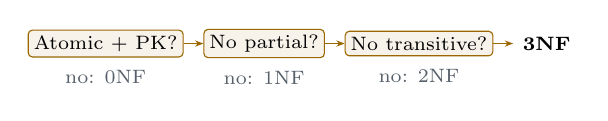
\begin{tikzpicture}[node distance=2.5mm, every node/.style={font=\scriptsize}]
  \node[draw=norm, fill=norm!8, rounded corners=1.5pt, inner sep=2pt] (a) {Atomic + PK?};
  \node[draw=norm, fill=norm!8, rounded corners=1.5pt, inner sep=2pt, right=of a] (b) {No partial?};
  \node[draw=norm, fill=norm!8, rounded corners=1.5pt, inner sep=2pt, right=of b] (c) {No transitive?};
  \node[right=of c, font=\scriptsize\bfseries] (d) {3NF};
  \draw[-{Stealth[length=3pt]}, norm] (a) -- (b);
  \draw[-{Stealth[length=3pt]}, norm] (b) -- (c);
  \draw[-{Stealth[length=3pt]}, norm] (c) -- (d);
  \node[below=1pt of a, color=muted] {no: 0NF};
  \node[below=1pt of b, color=muted] {no: 1NF};
  \node[below=1pt of c, color=muted] {no: 2NF};
\end{tikzpicture}

\begin{trap}
Test dependencies \textbf{on the data}: find two rows with the same $X$; different $Y$ means $X \not\to Y$. Ignore column order, and never use names as keys (two different patients are both ``Mary Smith'').
\end{trap}
\begin{trap}
A column with gaps in the data is optional \code{[col]}. An m:n pair (book with two authors, author with two books) needs its own table.
\end{trap}
\end{topic}

% ================================================================ SQL
\begin{topic}{sql}{4 \quad SQL: DDL and DML}
\sub[sql]{RMap to CREATE TABLE}
\begin{tabularx}{\linewidth}{@{}l X@{}}
underlined key & \code{PRIMARY KEY} / \code{PRIMARY KEY (a, b)} \\
no brackets & \code{NOT NULL} \\
\code{[brackets]} & leave \code{NOT NULL} off \\
underlined, not PK & \code{UNIQUE} \\
dashed arrow & \code{FOREIGN KEY (c) REFERENCES T(c)} \\
fixed list & \code{ENUM('A', 'B')} \\
generated number & \code{INT AUTO\_INCREMENT} \\
\end{tabularx}
\begin{lstlisting}
CREATE TABLE Booking (
  memberID  VARCHAR(5) NOT NULL,
  classCode VARCHAR(6) NOT NULL,
  bookedOn  DATE       NOT NULL,
  PRIMARY KEY (memberID, classCode),
  FOREIGN KEY (memberID)  REFERENCES Member(memberID),
  FOREIGN KEY (classCode) REFERENCES Class(classCode));
ALTER TABLE Member ADD COLUMN tier ENUM('Std','Pro');
\end{lstlisting}
Create parents first; drop children first.

\sub[sql]{DML}
\begin{lstlisting}
INSERT INTO Member VALUES ('M04','Dan Ho',NULL,'d@m.com');
INSERT INTO Member (memberID, memberName, email)
  VALUES ('M05','Eve Lam','e@m.com');
UPDATE Member SET phoneNo = '0400' WHERE memberID = 'M02';
DELETE FROM Booking WHERE memberID = 'M03';
\end{lstlisting}

\sub[sql]{Will this INSERT run? Check in order}
\textbf{PK} duplicate? $\;\to\;$ \textbf{FK} parent exists? $\;\to\;$ \textbf{UNIQUE} taken? $\;\to\;$ \textbf{NOT NULL} missing? $\;\to\;$ \textbf{ENUM} allowed value? Deleting a parent with child rows also fails.
\end{topic}

\begin{topic}{sql}{4 \quad SQL: queries}
\sub[sql]{Execution order}
\textbf{FROM/JOIN} $\to$ \textbf{WHERE} $\to$ \textbf{GROUP BY} $\to$ \textbf{HAVING} $\to$ \textbf{SELECT} $\to$ \textbf{ORDER BY}

\sub[sql]{Operators}
\code{IN (...)}, \code{BETWEEN a AND b} (inclusive), \code{LIKE 'C\%'} (\code{\%} any, \code{\_} one), \code{IS NULL}, \code{DISTINCT}, \code{ORDER BY c DESC}.

\sub[sql]{Aggregates}
\begin{lstlisting}
SELECT customerID, SUM(totalPrice) AS spent
FROM Orders
GROUP BY customerID
HAVING SUM(totalPrice) > 100;
\end{lstlisting}
\begin{itemize}
  \item WHERE filters rows; HAVING filters groups.
  \item \code{COUNT(*)} counts rows; \code{COUNT(col)} skips NULLs.
  \item Non-aggregated SELECT columns go in GROUP BY.
\end{itemize}

\sub[sql]{Joins}
\begin{lstlisting}
SELECT m.memberName FROM Member m
LEFT JOIN Booking b ON m.memberID = b.memberID
WHERE b.classCode IS NULL;   -- never booked
\end{lstlisting}
INNER keeps matches only. LEFT keeps every left row; unmatched right columns are NULL.

\sub[sql]{Subqueries and set operators}
\begin{lstlisting}
SELECT className FROM Class WHERE classCode NOT IN
  (SELECT classCode FROM Booking WHERE memberID = 'M01');
SELECT memberID FROM Member
EXCEPT SELECT memberID FROM Booking;
\end{lstlisting}
Read nested \code{IN} from the inside out. \code{UNION} removes duplicates, \code{UNION ALL} keeps them, \code{EXCEPT} subtracts. Same number of columns on both sides.
\end{topic}

\begin{topic}{sql}{4 \quad SQL: TCL and DCL}
\begin{lstlisting}
START TRANSACTION;
UPDATE Member SET phoneNo = '0499' WHERE memberID = 'M04';
COMMIT;   -- or ROLLBACK;
CREATE ROLE 'frontdesk';
GRANT SELECT ON fithub.* TO 'frontdesk';
GRANT INSERT, UPDATE ON fithub.Booking TO 'frontdesk';
GRANT 'frontdesk' TO 'sam'@'localhost';
SET DEFAULT ROLE ALL TO 'sam'@'localhost';
REVOKE UPDATE ON fithub.Booking FROM 'frontdesk';
\end{lstlisting}
Two roles = union of privileges. Add/edit but not remove: grant \code{SELECT, INSERT, UPDATE}, no \code{DELETE}.
\begin{trap}
\code{CREATE}, \code{ALTER}, \code{DROP} commit automatically. A later \code{ROLLBACK} can't undo anything before them.
\end{trap}
\end{topic}

\end{multicols*}
\end{document}
